\documentclass[letterpaper,openany,oneside,twocolumn]{book}

\newcommand{\PATH}{../../}

\usepackage{fontspec}
\usepackage[justified]{\PATH dndtemplate/dnd}
\usepackage{ifthen}
\usepackage{pstricks}

\usepackage{intcalc}

\usepackage[UKenglish]{babel}
\usepackage{\PATH dndtemplate}

\setlength\oddsidemargin{\dimexpr(\paperwidth-\textwidth)/2 - 1in\relax}
\setlength\evensidemargin{\oddsidemargin}

% Headline
\CharacterName{Alistair Hellstrum}

\Class{Bard}
\Level{4}
\Background{Courtier}
\PlayerName{M4RZ}
\Race{Tiefling}
\Alignment{Chaotic Good}
\XP{}

% Ability scores (correct scores, no modifiers are automatically applied)
% Modifiers, Saving Throws and Skills are calculated automatically
\StrengthScore{10}
\DexterityScore{16}
\ConstitutionScore{12}
\IntelligenceScore{12}
\WisdomScore{12}
\CharismaScore{18}

% Proficiencies (Proficient = 'P', Expertise = 'E', otherwise = '')
\StrengthProficiency{}
\DexterityProficiency{P}
\ConstitutionProficiency{}
\IntelligenceProficiency{}
\WisdomProficiency{}
\CharismaProficiency{P}

\AcrobaticsProficiency{P}
\AnimalHandlingProficiency{}
\ArcanaProficiency{P}
\AthleticsProficiency{}
\DeceptionProficiency{E}
\HistoryProficiency{P}
\InsightProficiency{P}
\IntimidationProficiency{P}
\InvestigationProficiency{}
\MedicineProficiency{}
\NatureProficiency{}
\PerceptionProficiency{}
\PerformanceProficiency{E}
\PersuasionProficiency{E} % Courtier Background
\ReligionProficiency{}
\SleightOfHandProficiency{}
\StealthProficiency{}
\SurvivalProficiency{}

\Inspiration{}
\Proficiency{+2}

% Armor Class is not automatically calculated
\ArmorClass{\intcalcAdd{11}{\calculateModifier{\DexterityScoreValue}}}
\InitiativeModifier{0}
\Speed{30ft}
\MaxHitPointsRolled{27} % Without Constitution Bonus, is added automatically
\CurrentHitPoints{}
\TemporaryHitPoints{}
\HitDice{d8}
\HitDiceSpent{0}

\CP{}
\SP{}
\EP{}
\GP{255}
\PP{}

% Weapon Arsenal
\AddWeapon{Rapier}{0}{1d8 p}
\AddWeapon{Dagger}{0}{1d4 p}

\AttacksAdditional{
	\textbf{Rapier}, \textbf{Dagger}\\
	\textbf{Armor:}
	\begin{itemize}
		\item Leather Armor
	\end{itemize}
}

\OtherProficienciesLanguages{
\textbf{Languages:}\\Common, Infernal\\
\textbf{Armor:}\\Light Armor\\
\textbf{Weapons:}\\Simple Weapons, Hand Crossbows, Longswords, Rapiers, Shortswords\\
\textbf{Tools:}\\Bagpipe, Lure, Violin
}

\Equipment{
	a backpack, a bedroll, 2 costumes, 5 candles, 5 days of ration, a waterskin, a disguise kit\\
	\textbf{Violin}, \textbf{Eliwick's blank sheet of paper}\\
	1 ruby (medium), 1 sapphire (medium)
}

\PersonalityTraits{
	\textbf{Charismatic:} Alistair possesses a natural charm and magnetic personality that draws people to him. He has a way with words and a captivating presence that allows him to easily connect with others.
}

\Ideals{
	\textbf{Musical Legacy:} Alistair is deeply connected to his musical heritage. He carries the weight of his family's musical lineage and strives to honor their legacy through his performances.
}

\Bonds{
	\textbf{Freedom of Expression:} Alistair believes in the power of artistic expression as a means of personal and societal liberation.
}

\Flaws{
	\textbf{Impulsive:} Alistair's passionate nature sometimes leads him to act on impulse, without considering the potential consequences.
}

\FeaturesTraits{
\textbf{Tiefling Traits}
\begin{itemize}
	\item Darkvision
	\item Hellish Resistance
	\item Infernal Legacy
\end{itemize}
\textbf{Court Functionary}\\
\textbf{Silver Tongued}
\begin{itemize}
	\item Charismatic Presence
	\item Charming Words
	\item Eloquent Performer
\end{itemize}
\textbf{Bard}
\begin{itemize}
	\item Bardic Inspiration
	\item Jack-of-All-Trades
	\item Song of Rest
	\item Bard College of Whispers
	\begin{itemize}
		\item Psychic Blades
		\item Words of Terror
	\end{itemize}
\end{itemize}
\textbf{Charm of the Monarch}\\
\textbf{Compulsion (Locket)}
\begin{itemize}
	\item CHA-Checks +1
\end{itemize}
}

% Appearance

\Age{34}
\Height{6'1}
\Weight{150lbs}
\Eyes{Golden-Amber}
\Skin{Burgundy}
\Hair{Black}

% background

\CharacterAppearance{}{
	\hspace*{-1.5em}\begin{tabular}{p{90pt}p{75pt}}
		\begin{tabular}{p{90pt}}\vspace*{-2em}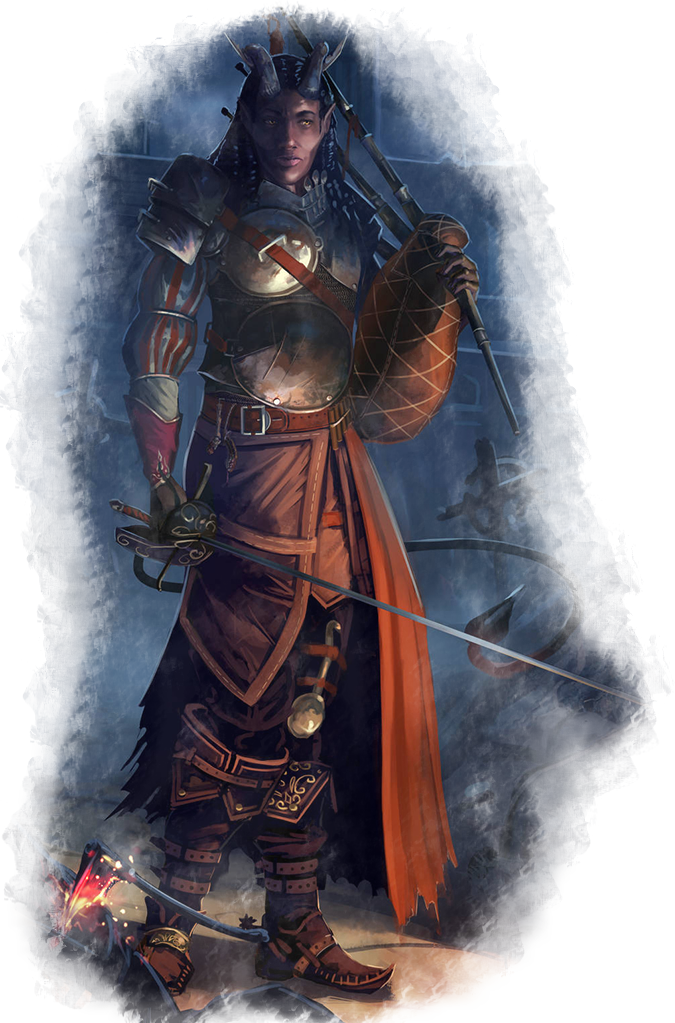
\includegraphics[width=100pt, height=140pt, keepaspectratio]{images/Alistair_appearance.png}\end{tabular}
		&
		\hspace*{-0.95em}\begin{tabular}{p{75pt}}Alistair Hellstrum stands at an average height with a lean and agile build. His skin has a rich, deep burgundy hue, a testament to his infernal heritage as a Tiefling. His eyes are a striking shade of golden ~~~~~~~~~\end{tabular}
	\end{tabular}\\\vspace*{-1.6em}\hfill\\
	amber, shimmering with a mischievous glint and an air of confidence. Alistair's dark, wavy hair cascades down to his shoulders, accentuating his charismatic and somewhat untamed demeanor.
}{}{}{}
\AdditionalFeaturesAndTraits{
	Alistair is not only a skilled musician but also a versatile performer. He excels in various forms of artistic expression, including acting, storytelling, and dancing. His performances are captivating and immersive, captivating audiences with their richness and variety.\\
	Alistair has a talent for languages and has devoted time to learning and mastering multiple tongues. In addition to Common and Infernal, he may be fluent in Elvish, Dwarvish, or other languages he has encountered during his travels. This linguistic ability allows him to connect with diverse cultures and communicate effectively with a wide range of individuals.\\
	Alistair has developed impressive negotiation skills over the years. He can find common ground and resolve conflicts through diplomacy and tact. His silver tongue, combined with his ability to read people, gives him an advantage in navigating delicate social and political situations.\\
	Alistair has a keen interest in the arcane arts and has studied magical theory and lore. Though not a full-fledged spellcaster, he possesses a solid understanding of magic and can identify magical items, comprehend magical writings, and recognize spells being cast.
}
\Characterbackground{
	Alistair Hellstrum's journey began in a bustling port city, where he was born to a humble family. From a young age, Alistair showed a natural inclination towards music and performance. He would often spend his days enchanting passersby with his melodious voice and captivating tunes, earning him a few copper coins to help support his family.
	
	However, life in the city was not without its challenges. Alistair's Tiefling heritage made him a target of prejudice and mistrust from some of the city's residents. Determined to rise above the discrimination, Alistair honed his talents, pouring his heart and soul into his music. His enchanting performances became a beacon of hope and inspiration for others who faced similar struggles.
	
	With his silver tongue, mesmerizing melodies, and unwavering spirit, Alistair Hellstrum, the Tiefling Bard, carries the torch of hope and harmony wherever his journey takes him.
}
\Treasure{
	\textbf{1. Ancient Manuscript:} Alistair possesses a weathered and meticulously preserved manuscript filled with ancient songs, stories, and forgotten lore. The pages are yellowed with age, and delicate illustrations adorn its margins. This precious relic is a treasure trove of inspiration, containing forgotten melodies, tales of legendary heroes, and cryptic clues that hint at hidden places of power.\\
	\textbf{2. Curious Relic (The Enchanted Locket of Lysandra):} Alistair possesses a peculiar relic, a seemingly ordinary, unadorned silver locket on a delicate chain. To the casual observer, it looks like an ordinary piece of jewelry with no special significance. However, upon closer inspection, faint, ever-shifting patterns of light dance across its surface, hinting at its magical nature.\\
	Unbeknownst to Alistair it kindles an insatiable fascination with the Fewild, which becomes stronger the more he interacts with the Feywild and its creatures.
}
\AlliesAndOrganizations{
	Most folk are happy to welcome a bard into their midst. Bards of the College of Whispers use this to their advantage. They appear to be like any other bard, sharing news, singing songs, and telling tales to the audiences they gather. In truth, the College of Whispers teaches its students that they are wolves among sheep. These bards use their knowledge and magic to uncover secrets and turn them against others through extortion and threats.

	Many other bards hate the College of Whispers, viewing it as a parasite that uses the bards' reputation to acquire wealth and power. For this reason, these bards rarely\linebreak
}{
	reveal their true nature unless they must. They typically claim to follow some other college, or keep their true nature secret in order to better infiltrate and exploit royal courts and other settings of power.
}
\OrganizationName{Bard College of Whispers}
\OrganizationSymbol{images/Bard_College_of_Lore.png}

% Magic

\SpellcastingClass{Bard}
\SpellcastingAbility{CHA} % STR, DEX, CON, INT, WIS, CHA
\SpellSaveDCModifier{0} % any modifier that isn't contained in "8 + Ability Modifier + Proficiency Bonus"

\CantripSlotA{Mage Hand (V, S)}
\CantripSlotB{Prestidigitation (V, S)}
\CantripSlotC{Vicious Mockery (V)}
\CantripSlotD{Thaumaturgy (once per day) (V)}

\FirstLevelSpellSlotsTotal{4}
\FirstLevelSpellSlotA{Charm Person (V, S)}
\FirstLevelSpellSlotB{Dissonant Whispers (V)}
\FirstLevelSpellSlotC{Faerie Fire (V)}
\FirstLevelSpellSlotD{Healing Word (V)}
\FirstLevelSpellSlotE{Hellish Rebuke (once per day) (V, S)}

\SecondLevelSpellSlotsTotal{3}
\SecondLevelSpellSlotA{Invisibility (V, S, M)}
\SecondLevelSpellSlotB{Shatter (V, S, M)}
\SecondLevelSpellSlotC{Suggestion (V, M)}

\begin{document}

\newgeometry{left=0cm,right=0cm,top=0cm,bottom=0cm}
\onecolumn


% CHARACTER PAGE
\rendercharactersheet

% BACKSTORY PAGE
\renderbackgroundsheet

% SPELLCASTING PAGE
\renderspellsheet


\restoregeometry
\twocolumn

\chapter*{Recent Backstory}

{\noindent \entryfont \DndDropCapLine{A}listair, a talented and curious Tiefling bard, led a life of modest contentment. He wandered through towns and villages, sharing his songs and stories with eager audiences, unaware of the mystical wonders that lay beyond the realm of his knowledge. Little did he know that his fate was about to take an enchanting turn. He had performed for kings and peasants alike, honing his bardic talents and captivating audiences with stories of far-off lands.

One fateful day, while traversing a dense forest, Alistair's path led him to a secluded glade untouched by time. There, nestled amidst a bed of vibrant wildflowers, lay a silver locket, emitting a faint, otherworldly glow. Intrigued, he picked it up, feeling an immediate connection - a pulse of magic that resonated deep within his being. Alistair was slowly but steadily overcome by a rush of inexplicable emotions, as if the locket had awakened a part of him he never knew existed.

As the locket's magic flowed through him, Alistair's perception of the world began to shift. Vivid dreams of the Feywild's ethereal landscapes filled his nights, drawing him into a realm of enchantment and whimsy. The locket's melodies echoed in his mind, its whispers of the Feywild's beauty and mystery becoming a siren's call that he could not ignore.\\

\paragraph*{A Peculiar Encounter} During his newfound journey of discovery, Alistair's path crossed with that of a peculiar cleric named Alaric Kain. Known not only for his devotion to his deity but also for his insatiable cleptomania, Alaric was a charismatic individual with a penchant for getting into and especially out of trouble.

Their meeting was far from cordial. One serene afternoon, Alistair discovered Alaric attempting to pilfer a trinket from his belongings. Swift as a breeze, Alistair caught the cleric in the act, their gazes locking in a tense standoff. The air crackled with tension as Alistair demanded an explanation for the attempted theft. Alaric, undeterred, smirked and admitted his intent, claiming that he had sensed the locket's magical energy and was driven to understand its potential.

Despite the initial confrontation, Alistair's curiosity led him to strike an unlikely alliance with Alaric. Recognizing that they both harbored a burning desire to reach the Feywild, they decided to set aside their differences. While Alistair was wary of Alaric's tendencies, the shared goal of uncovering the mysteries of the Feywild provided a common purpose that bound them together.

As Alistair and Alaric journeyed together, their dynamic was a mix of camaraderie and tension. Alistair held the locket close, his attachment unbreakable, while Alaric's kleptomania occasionally caused friction. Yet, the shared goal of reaching the Feywild acted as a beacon, guiding them through challenges and obstacles.

\eject

\paragraph*{Enchanting Carnival} Their path eventually led them to a new destination - the Witchlight Carnival. The sound of music and laughter filled the air as they approached, signaling the arrival of the carnival. For Alistair and Alaric, this was not just another carnival - it was a stepping stone on their journey to the Feywild, a realm of dreams and mysteries waiting to be unveiled.

As they entered the carnival's enchanting realm, they were both acutely aware that their alliance held the potential to lead them to the heart of the Feywild itself. The locket's whispering enchantment was a constant reminder of the destiny that awaited them - one of discovery, danger, and the intertwining of their fates.

And so, under the starlit sky, Alistair and Alaric explored their surroundings, united by the allure of the Feywild and the shared pursuit of the mysteries behind the Enchanted Locket of Lysandra. At the Witchlight Carnival their journey was about to take an unexpected turn, where the lines between reality and enchantment would blur, and the whimsy of the Feywild would guide them toward their destiny.
}

\clearpage

\chapter*{Features, Magic Items and Spells}

\section*{Tiefling Traits}
\subsection*{Darkvision}
Thanks to your infernal heritage, you have superior vision in dark and dim conditions. You can see in dim light within 60 feet of you as if it were bright light, and in darkness as if it were dim light. You can’t discern color in darkness, only shades of gray.
\subsection*{Hellish Resistance}
You have resistance to fire damage.
\subsection*{Infernal Legacy}
You know the Thaumaturgy cantrip. Once you reach 3rd level, you can cast the Hellish Rebuke spell once as a 2nd-level spell. Once you reach 5th level, you can also cast the Darkness spell once. You must finish a long rest to cast these spells again with this trait. Charisma is your spellcasting ability for these spells.

\section*{Court Functionary}
Your knowledge of how bureaucracies function lets you gain access to the records and inner workings of any noble court or government you encounter. You know who the movers and shakers are, whom to go to for the favors you seek, and what the current intrigues of interest in the group are.

\section*{Silver Tongued}
\subsection*{Charismatic Presence}
You gain proficiency in the Persuasion skill if you don't already have it. If you already have proficiency in Persuasion, you gain expertise in that skill, doubling your proficiency bonus for ability checks made with it.
\subsection*{Charming Words}
You can spend 10 minutes engaging in conversation with a creature you can see, and if the creature's Intelligence is 6 or higher, you can attempt to charm it. Make a Charisma (Persuasion) check contested by the creature's Wisdom saving throw. If you succeed, the creature becomes charmed by you for 1 hour or until you or your companions harm it. The DM determines the specifics of the creature's behavior while charmed.
\subsection*{Eloquent Performer}
When you use the Performance skill to entertain, inspire, or captivate an audience, your performance is exceptionally compelling. You have advantage on Performance checks made to impress or engage a crowd.

\section*{Bard}
\subsection*{Bardic Inspiration}
You can inspire others through stirring words or music. To do so, you use a bonus action on your turn to choose one creature other than yourself within 60 feet of you who can hear you. That creature gains one Bardic Inspiration die, a d6.

Once within the next 10 minutes, the creature can roll the die and add the number rolled to one ability check, attack roll, or saving throw it makes. The creature can wait until after it rolls the d20 before deciding to use the Bardic Inspiration die, but must decide before the DM says whether the roll succeeds or fails. Once the Bardic Inspiration die is rolled, it is lost. A creature can have only one Bardic Inspiration die at a time.

You can use this feature a number of times equal to your Charisma modifier (a minimum of once). You regain any expended uses when you finish a long rest.

Your Bardic Inspiration die changes when you reach certain levels in this class. The die becomes a d8 at 5th level, a d10 at 10th level, and a d12 at 15th level.

(\textbf{Usages: \intcalcAdd{0}{\calculateModifier{\CharismaScoreValue}}})
\subsection*{Jack-of-All-Trades}
Starting at 2nd level, you can add half your proficiency bonus, rounded down, to any ability check you make that doesn't already include your proficiency bonus.
\subsection*{Song of Rest}
Beginning at 2nd level, you can use soothing music or oration to help revitalize your wounded allies during a short rest. If you or any friendly creatures who can hear your performance regain hit points at the end of the short rest by spending one or more Hit Dice, each of those creatures regains an extra 1d6 hit points.

The extra Hit Points increase when you reach certain levels in this class: to 1d8 at 9th level, to 1d10 at 13th level, and to 1d12 at 17th level.
\subsection*{Bard College of Whispers}
\subsubsection*{Psychic Blades}
When you join the College of Whispers at 3rd level, you gain the ability to make your weapon attacks magically toxic to a creature's mind.

When you hit a creature with a weapon attack, you can expend one use of your Bardic Inspiration to deal an additional 2d6 psychic damage to that target. You can do so only once per round on your turn.

The psychic damage increases when you reach certain levels in this class, increasing to 3d6 at 5th level, 5d6 at 10th level, and 8d6 at 15th level.

\subsubsection*{Words of Terror}
At 3rd level, you learn to infuse innocent-seeming words with an insidious magic that can inspire terror.

If you speak to a humanoid alone for at least 1 minute, you can attempt to seed paranoia and fear into its mind. At the end of the conversation, the target must succeed on a Wisdom saving throw against your spell save DC or be frightened of you or another creature of your choice. The target is frightened in this way for 1 hour, until it is attacked or damaged, or until it witnesses its allies being attacked or damaged.

If the target succeeds on its saving throw, the target has no hint that you tried to frighten it.

Once you use this feature, you can't use it again until you finish a short rest or long rest.
\subsection*{Charm of the Monarch}
You can sprout a pair of beautiful butterfly wings, you gain flying speed equal to your walking speed, and you gain a +5 bonus on all Charisma-based ability checks. These effects last for 1 hour. After you use this charm two times, it vanishes from you.\\
\textbf{(Usages: 1)}

\section*{Spells}
\subsection*{Cantrip}

\DndSpellHeader
  {Mage Hand}
  {Cantrip Conjuration}
  {1 Action}
  {30 feet}
  {V, S}
  {1 Minute}
  
A spectral, floating hand appears at a point you choose within range. The hand lasts for the duration or until you dismiss it as an action. The hand vanishes if it is ever more than 30 feet away from you or if you cast this spell again.\\
You can use your action to control the hand. You can use the hand to manipulate an object, open an unlocked door or container, stow or retrieve an item from an open container, or pour the contents out of a vial. You can move the hand up to 30 feet each time you use it.\\
The hand can’t attack, activate magic items, or carry more than 10 pounds.

\DndSpellHeader
  {Prestidigitation}
  {Cantrip Transmutation}
  {1 Action}
  {10 feet}
  {V, S}
  {Up to 1 hour}

This spell is a minor magical trick that novice spellcasters use for practice. You create one of the following magical effects within range:\\
You create an instantaneous, harmless sensory effect, such as a shower of sparks, a puff of wind, faint musical notes, or an odd odor.\\
You instantaneously light or snuff out a candle, a torch, or a small campfire.\\
You instantaneously clean or soil an object no larger than 1 cubic foot.\\
You chill, warm, or flavor up to 1 cubic foot of nonliving material for 1 hour.\\
You make a color, a small mark, or a symbol appear on an object or a surface for 1 hour.\\
You create a nonmagical trinket or an illusory image that can fit in your hand and that lasts until the end of your next turn.\\
If you cast this spell multiple times, you can have up to three of its non-instantaneous effects active at a time, and you can dismiss such an effect as an action.

\DndSpellHeader
  {Vicious Mockery}
  {Cantrip Enchantment}
  {1 Action}
  {A creature you can see and that can hear you within range}
  {V}
  {Instantaneous}

You unleash a string of insults laced with subtle enchantments at a creature you can see within range. If the target can hear you (though it need not understand you), it must succeed on a Wisdom saving throw or take \DndDice{1d4} psychic damage and have disadvantage on the next attack roll it makes before the end of its next turn.

\DndSpellHeader
  {Thaumaturgy}
  {Cantrip Transmutation}
  {1 Action}
  {30 feet}
  {V}
  {Up to 1 minute}

You manifest a minor wonder, a sign of supernatural power create one of the following magical effects within range:\\
Your voice booms up to three times as loud as normal for 1 minute.\\
You cause flames to flicker, brighten, dim, or change color for 1 minute.\\
You cause harmless tremors in the ground for 1 minute.\\
You create an instantaneous sound that originates from a point of your choice within range, such as a rumble of thunder.\\
You instantaneously cause an unlocked door or window to fly open or slam shut.\\
You alter the appearance of your eyes for 1 minute.\\
If you cast this spell multiple times, you can have up to three of its effects active at a time, and you can dismiss such an effect as an action.\\

\subsection*{Level 1}

\DndSpellHeader
  {Charm Person}
  {1st Level Enchantment}
  {1 Action}
  {30 feet}
  {V, S}
  {1 hour}

You attempt to charm a humanoid you can see within range. It must make a Wisdom saving throw, and does so with advantage if you or your companions are fighting it. If it fails the saving throw, it is charmed by you until the spell ends or until you or your companions do anything harmful to it. The charmed creature regards you as a friendly acquaintance. When the spell ends, the creature knows it was charmed by you.

\subparagraph*{At Higher Levels} When you cast this spell using a spell slot of 2nd level or higher, you can target one additional creature for each slot level above 1st. The creatures must be within 30 feet of each other when you target them.

\DndSpellHeader
  {Dissonant Whispers}
  {1st Level Enchantment}
  {1 Action}
  {60 feet}
  {V}
  {Instantaneous}

You whisper a discordant melody that only one creature of your choice within range can hear, wracking it with terrible pain. The target must make a Wisdom saving throw. On a failed save, it takes \DndDice{3d6} psychic damage and must immediately use its reaction, if available, to move as far as its speed allows away from you. The creature doesn’t move into obviously dangerous ground, such as a fire or a pit. On a successful save, the target takes half as much damage and doesn’t have to move away. A deafened creature automatically succeeds on the save.

\subparagraph*{At Higher Levels} When you cast this spell using a spell slot of 2nd level or higher, the damage increases by \DndDice{1d6} for each slot level above 1st.

\DndSpellHeader
  {Faerie Fire}
  {1st-Level Evocation}
  {1 Action}
  {60 feet}
  {V}
  {Concentration, up to 1 minute}

Each object in a 20-foot cube within range is outlined in blue, green, or violet light (your choice). Any creature in the area when the spell is cast is also outlined in light if it fails a Dexterity saving throw. For the duration, objects and affected creatures shed dim light in a 10-foot radius.

Any attack roll against an affected creature or object has advantage if the attacker can see it, and the affected creature or object can't benefit from being invisible.

\DndSpellHeader
  {Healing Word}
  {1st Level Evocation}
  {1 Bonus Action}
  {60 feet}
  {V}
  {Instantaneous}

A creature of your choice that you can see within range regains hit points equal to \DndDice{1d4} + your spellcasting ability modifier \textbf{(+\intcalcAdd{0}{\calculateModifier{\CharismaScoreValue}})}. This spell has no effect on undead or constructs.

\subparagraph*{At Higher Levels} When you cast this spell using a spell slot of 2nd level or higher, the Healing increases by \DndDice{1d4} for each slot level above 1st.

\DndSpellHeader
  {Hellish Rebuke}
  {1st Level Evocation}
  {1 Reaction, which you take in response to being damaged by a creature within 60 feet of you that you can see}
  {60 feet}
  {V, S}
  {Instantaneous}

You point your finger, and the creature that damaged you is momentarily surrounded by hellish flames. The creature must make a Dexterity saving throw. It takes \DndDice{2d10} fire damage on a failed save, or half as much damage on a successful one.

\subparagraph*{At Higher Levels} When you cast this spell using a spell slot of 2nd level or higher, the damage increases by \DndDice{1d10} for each slot level above 1st.

\subsection*{Level 2}

\DndSpellHeader
  {Invisibility}
  {2nd Level Illusion}
  {1 Action}
  {Touch}
  {V, S, M (An eyelash encased in gum arabic)}
  {Concentration, Up to 1 Hour}
  
A creature you touch becomes invisible until the spell ends. Anything the target is wearing or carrying is invisible as long as it is on the target’s person. The spell ends for a target that attacks or casts a spell.

\subparagraph*{At Higher Levels} When you cast this spell using a spell slot of 3rd level or higher, you can target one additional creature for each slot level above 2nd.

\DndSpellHeader
  {Shatter}
  {2nd Level Evocation}
  {1 Action}
  {60 feet}
  {V, S, M (A chip of mica)}
  {Instantaneous}

A sudden loud ringing noise, painfully intense, erupts from a point of your choice within range. Each creature in a 10-foot-radius sphere centered on that point must make a Constitution saving throw. A creature takes \DndDice{3d8} thunder damage on a failed save, or half as much damage on a successful one. A creature made of inorganic material such as stone, crystal, or metal has disadvantage on this saving throw. A nonmagical object that isn’t being worn or carried also takes the damage if it’s in the spell’s area.

\subparagraph*{At Higher Levels} When you cast this spell using a spell slot of 3rd level or higher, the damage increases by \DndDice{1d8} for each slot level above 2nd.

\DndSpellHeader
  {Suggestion}
  {2nd Level Enchantment}
  {1 Action}
  {30 feet}
  {V, M (A snake's tongue and either a bit of honeycomb or a drop of sweet oil)}
  {Concentration, Up to 8 hours}

You suggest a course of activity (limited to a sentence or two) and magically influence a creature you can see within range that can hear and understand you. Creatures that can’t be charmed are immune to this effect. The suggestion must be worded in such a manner as to make the course of action sound reasonable. Asking the creature to stab itself, throw itself onto a spear, immolate itself, or do some other obviously harmful act ends the spell.\\
The target must make a Wisdom saving throw. On a failed save, it pursues the course of action you described to the best of its ability. The suggested course of action can continue for the entire duration. If the suggested activity can be completed in a shorter time, the spell ends when the subject finishes what it was asked to do.\\
You can also specify conditions that will trigger a special activity during the duration. For example, you might suggest that a knight give her warhorse to the first beggar she meets. If the condition isn’t met before the spell expires, the activity isn’t performed.\\
If you or any of your companions damage the target, the spell ends.

\section*{Miscellaneous}
\subsubsection*{Weapon Attacks}
\paragraph*{Attack Roll}\hfill\\
\underline{Rapier:}\\
1d20 + DEX-Modifier + Proficiency Modifier\\
\indent Current Max: \intcalcAdd{20}{\intcalcAdd{\calculateModifier{\DexterityScoreValue}}{\ProficiencyValue}}\\
\underline{Dagger:}\\
1d20 + DEX-Modifier + Proficiency Modifier\\
\indent Current Max: \intcalcAdd{20}{\intcalcAdd{\calculateModifier{\DexterityScoreValue}}{\ProficiencyValue}}\\
\paragraph*{Damage Roll}\hfill\\
\underline{Rapier:}\\
1d8 + DEX-Modifier (+2d6 Psychic Damage (Psychic Blades))\\
\indent Current Max (Normal): \intcalcAdd{8}{\calculateModifier{\DexterityScoreValue}}\\
\indent Current Max (Psychic Blades): \intcalcAdd{8}{\intcalcAdd{\calculateModifier{\DexterityScoreValue}}{\intcalcMul{2}{6}}}\\
\underline{Dagger:}\\
1d4 + DEX-Modifier (+2d6 Psychic Damage (Psychic Blades))\\
\indent Current Max (Normal): \intcalcAdd{4}{\calculateModifier{\DexterityScoreValue}}\\
\indent Current Max (Psychic Blades): \intcalcAdd{4}{\intcalcAdd{\calculateModifier{\DexterityScoreValue}}{\intcalcMul{2}{6}}}\\

\chapter*{The Enchanted Locket of Lysandra}
\begin{tikzpicture}[remember picture, overlay]
	\node[xshift=3cm, yshift=0.8cm] {\textit{Locket, rare (requires attunement)}};
	\node[xshift=3.5cm, yshift=-5cm] {
\includegraphics[width=1.3\columnwidth]{images/Locket_of_Lysandra.png}};
\end{tikzpicture}
\vspace*{10cm}
\section*{Appearance}
The Enchanted Locket of Lysandra appears as a simple and unadorned silver locket on a delicate chain. To the casual observer, it looks like an ordinary piece of jewelry with no special significance. However, upon closer inspection, however, the true magic of the locket becomes apparent. Faint, ever-shifting patterns of light dance across its surface like playful fireflies on a warm summer night. These ethereal luminescent swirls seem to weave intricate stories, their fleeting forms conjuring images of blooming wildflowers, starlit skies, and the elusive spirits of the Feywild. Each flicker of light holds a hint of forgotten tales, a connection to a realm of dreams that exists just beyond the veil of perception.

Adding to the intrigue, the locket possesses a set of minuscule, intricately wrought hinges that are barely discernible to the naked eye. These hinges, delicate as the gossamer wings of a butterfly, are an enigma in themselves, for they hint at the locket's potential to open and reveal its secrets. Yet, despite their apparent purpose, there is no physical means or any clue to unlocking the locket's hidden interior. It remains a tantalizing riddle, waiting for the touch of someone who holds both the key and the knowledge to unlock its mysteries.
\eject
\section*{History}
Legends speak of Lysandra, a powerful and enigmatic fey enchantress who once roamed the realms of Prismeer. Known for her boundless curiosity and mischievous nature, Lysandra was said to possess an item of unimaginable enchantment, capable of granting its bearer unparalleled insight into the secrets of the Feywild. The Enchanted Locket is believed to be a fragment of her lost legacy.
\vspace*{-1.2\fontdimen6\font}
\section*{Magic}
The locket has several magical properties, though Alistair might not be aware of all its abilities at the start of the campaign. As he uncover mores about the relic, he will discover its true potential. Some of its known abilities include:
\begin{itemize}
	\item \textbf{Fey Sensitivity:} The locket resonates with the energy of the Feywild, allowing its bearer to sense the presence of fey creatures and magical phenomena nearby. However, at times the holder becomes increasingly fixated on uncovering its secrets, neglecting other aspects of their life and their original quest. They might struggle to focus on anything else, including the well-being of their companions.
	\item \textbf{Dreams of the Fey:} When worn during sleep, the locket can grant visions and cryptic dreams about the Feywild, which become more unsettling as the influence of the locket grows.
	\item \textbf{Portal Attunement:} The locket can attune its bearer to specific Feywild locations, potentially serving as a key to unlock hidden pathways between the material world and the Feywild. But this bond could attract the attention of malevolent fey entities. These entities might attempt to manipulate or coerce your character into serving their own mysterious agendas.
	\item \textbf{Whisper of Lysandra:} In moments of uncertainty or danger, the locket may emit soft whispers of ancient Feywild wisdom, guiding its bearer's decisions - either helpful or malicious.
	\item \textbf{Mistrust of Mortals:} The locket's connection to the Feywild might foster a growing sense of alienation from the mortal world. The holder becomes more distant from non-fey creatures, finding it difficult to trust them.
	\item \textbf{Fading Identity:} As your character delves deeper into the locket's mysteries, they might find aspects of their identity beginning to blur. Memories of their life before the locket's influence become hazy, leading to a sense of disconnection from their past.
\end{itemize}
\section*{Compulsion}
The Enchanted Locket has a subtle yet powerful compulsion on its bearer. As your character carries the locket, its magic gradually influences their emotions and desires, kindling an insatiable fascination with the Feywild. The more they interact with the Feywild or embark on quests related to Prismeer, the stronger this compulsion becomes.

The locket's influence amplifies its bearer's natural magical inclinations, deepening his understanding of arcane secrets and Feywild lore. This newfound magical prowess enhances the Charismatic abilities of its bearer:
\begin{itemize}
	\item[$\ast$] \textbf{Level 4-6:} You gain a +1 bonus to Charisma ability checks while being attuned to the locket.
	\item \textbf{Level 7-11:} You gain a +2 bonus to Charisma ability checks and a -1 malus to Wisdom ability checks while being attuned to the locket.
	\item \textbf{Level 11-16:} You gain a +3 bonus to Charisma ability checks and a -1 malus to Wisdom ability checks while being attuned to the locket.
	\item \textbf{Level 17+:} You gain a +4 bonus to Charisma ability checks and a -2 malus to Wisdom ability checks while being attuned to the locket.
\end{itemize}
\section*{Curse of Whispered Entanglement}
The Enchanted Locket of Lysandra, despite its allure, carries a hidden curse that intertwines the bearer's fate with the whims of the Feywild. While the locket's charisma-enhancing effects are a boon, the Curse of Whispered Entanglement gradually begins to exert its influence, whispering subtle manipulations into the bearer's mind.

\paragraph*{Curse}
Once the character is attuned to this locket, he can not willingly unattune off it unless he is targeted by the remove curse spell or similar magic.

\paragraph{Compelled Decision}
Whenever a decision must be made or information is sought, the locket's magic compels the bearer to heed its suggestions. The Dungeon Master decides what the locket suggests in each situation. The bearer must succeed a Charisma Saving Throw for any decision the locket suggests or a Wisdom Saving Throw for any information the locket reveals. If the saving throw fails, the bearer is fully convinced by the locket's suggestion and feels compelled to act on it. If the saving throw is successful, the bearer can resist the locket's influence and make their own decision. The DC is increasing by the following means:
\eject
\begin{itemize}
	\item The Save DC starts at a value of 10
	\item With every successful Saving Throw regarding this effect the bearer makes the Save DC increases by \xdef\successIncrease{0.5}\successIncrease
	\item With every failed Saving Throw regarding this effect the bearer makes the Save DC increases by \xdef\failIncrease{0.25}\failIncrease
\end{itemize}
\textbf{Failed Saves:} \xdef\failedSaves{5}\failedSaves\\
\textbf{Successful Saves:} \xdef\successSaves{4}\successSaves\\
\textbf{Current Save DC: \FPeval{saveDC}{clip(10+\failedSaves*failIncrease+\successSaves*\successIncrease)}\saveDC}
\section*{Torn between Worlds}
While the locket provides Alistair with extraordinary insights and magical abilities, its influence comes at a cost. The more time he spends away from the Feywild or the locket, the more he feels an ache of longing and a sense of restlessness. Their connection with the locket intertwines his fate with that of the Feywild, making him feel incomplete whenever he is separated from it.
\section*{Quest of Discovery}
The Enigmatic Locket of Lysandra possesses an inherent, magical allure that captivates the heart and mind of Alistair, the Bard. When he first encountered the locket, he was drawn to it by an irresistible pull, not fully comprehending why it called to him so strongly. From that moment on, he found himself becoming increasingly obsessed with uncovering the locket's true nature and its connection to the Feywild.

\clearpage
\twocolumn[
	\section*{The Epic Adventures of the 7 Musceteers}\hfill\\\\\\
]
\newcommand{\chord}[1]{\colorbox{gray!60}{\footnotesize{#1}}}
\subsubsection*{Intro}
\chord{Am} \chord{F} \chord {Am} \chord{G}

\subsubsection*{Verse 1}
{\entryfont In Faerun's realm where legends gleam,}\\
A band of heroes, like in a dream,\\
Seven Musceteers, though five we stand,\\
Burro and Bob, wings of the land.\\
\\
Floppers the bunny, with dark arts crowned,\\
Raising the fallen, in necromancer's gown,\\
Kyuss, the spark of explosive might,\\
Burning through darkness, in the starry night.

\subsubsection*{Chorus}
\hspace*{1.5cm}\chord{Am}\hspace*{0.9cm}\chord{C}\hspace*{1cm}\chord{G}\hspace*{1.8cm}\chord{Dm}\\
{\entryfont These are days and nights of friendship and blood,}\\
\chord{Am}\hspace*{1.1cm}\chord{C}\hspace*{1.3cm}\chord{G}\hspace*{1.3cm}\chord{Em}\\
{\entryfont Heroes will rise as the \textbf{Storm} does fall,}\\
\chord{F}\hspace*{0.85cm}\chord{Am}\hspace*{0.4cm}\chord{G}\hspace*{1.3cm}\chord{Dm}\\
{\entryfont Side by side, a triumphant roar}\\
\hspace*{1.1cm}\chord{F}\hspace*{0.4cm}\chord{Em}\hspace*{1.9cm}\chord{Am}\\
{\entryfont In the heart of adventure, we ride.}

\subsubsection*{Interlude}
\chord{Am} \chord{F} \chord {Am} \chord{G} {\footnotesize x2}

\subsubsection*{Verse 2}
{\entryfont Stor the rogue, shadows his guide,}\\
Silent and quick, through danger we glide,\\
Jun Wu, the monk, fists pure and fast,\\
In pursuit of truth, our futures cast.\\
\\
Laucian the ranger, nature's embrace,\\
Guiding our steps through each sacred place,\\
Seven Musceteers, united we roam,\\
Heroes of honor, making Earth our home.

\subsubsection*{Chorus}
\hspace*{1.5cm}\chord{Am}\hspace*{0.9cm}\chord{C}\hspace*{1cm}\chord{G}\hspace*{1.8cm}\chord{Dm}\\
{\entryfont These are days and nights of friendship and blood,}\\
\chord{Am}\hspace*{1.1cm}\chord{C}\hspace*{1.3cm}\chord{G}\hspace*{1.3cm}\chord{Em}\\
{\entryfont Heroes will rise as the \textbf{Storm} does fall,}\\
\chord{F}\hspace*{0.85cm}\chord{Am}\hspace*{0.4cm}\chord{G}\hspace*{1.3cm}\chord{Dm}\\
{\entryfont Side by side, a triumphant roar}\\
\hspace*{1.1cm}\chord{F}\hspace*{0.4cm}\chord{Em}\hspace*{1.9cm}\chord{Am}\\
{\entryfont In the heart of adventure, we ride.}
\vfill\eject

\subsubsection*{Chorus}
{\entryfont Seven Musceteers, banners high,}\\
Facing down dragons in the endless sky,\\
Savage Frontier knows peace's embrace,\\
In our quest for justice, we find our grace.

\subsubsection*{Verse 3}
\entryfont Iymrith's end, a triumphant roar,\\
Defeating the Doom that plagued us before,\\
G\&G's Trading Post, flames in the night,\\
Justice pursued, but evading their sight.\\\\
Fire Giants' kinship, a bond that's been sealed,\\
Honorary titles in a powerful guild,\\
Seven Musceteers, forever they stand,\\
In the annals of time, their tale becomes grand.

\subsubsection*{Chorus}
\entryfont Seven Musceteers, journey complete,\\
A chorus of triumphs and battles' beat,\\
In taverns and halls, their stories are told,\\
Of heroes so valiant, and friendships so bold.

\subsubsection*{Endverse}
So lift your voices, let tales resound,\\
Of Musceteers bold, in quests unbound,\\
In songs and cheers, their legends ignite,\\
The Seven Musceteers, a shining light.
\vfill

\end{document}
